\documentclass{article}
\usepackage{epsf}
\usepackage{graphicx}
\usepackage{psfig}
\begin{document}

\begin{figure}
\epsffile{figtest.eps}
\caption{Figure test using epsffile.} 
\label{figure1}
\end{figure}

Figure \ref{figure1} tests \verb#\epsffile{figtest.eps}#.

\begin{figure*}
\epsffile{figtest.eps}
\caption{Figure* test using epsffile.} 
\label{figure1a}
\end{figure*}

Figure \ref{figure1} tests \verb#\epsffile{figtest.eps}#.

\begin{figure}

\includegraphics{figtest.eps}
\caption{Figure test using includegraphics.} 
\label{figure2}
\end{figure}

Figure \ref{figure2} tests \verb#\includegraphic{figtest.eps}#.

\begin{figure}
\psfig{figure=figtest.eps}
\caption{Figure test using psfig.} 
\label{figure3}
\end{figure}

Figure \ref{figure3} tests \verb#\psfig{figure=figtest.eps}#.

\begin{figure}
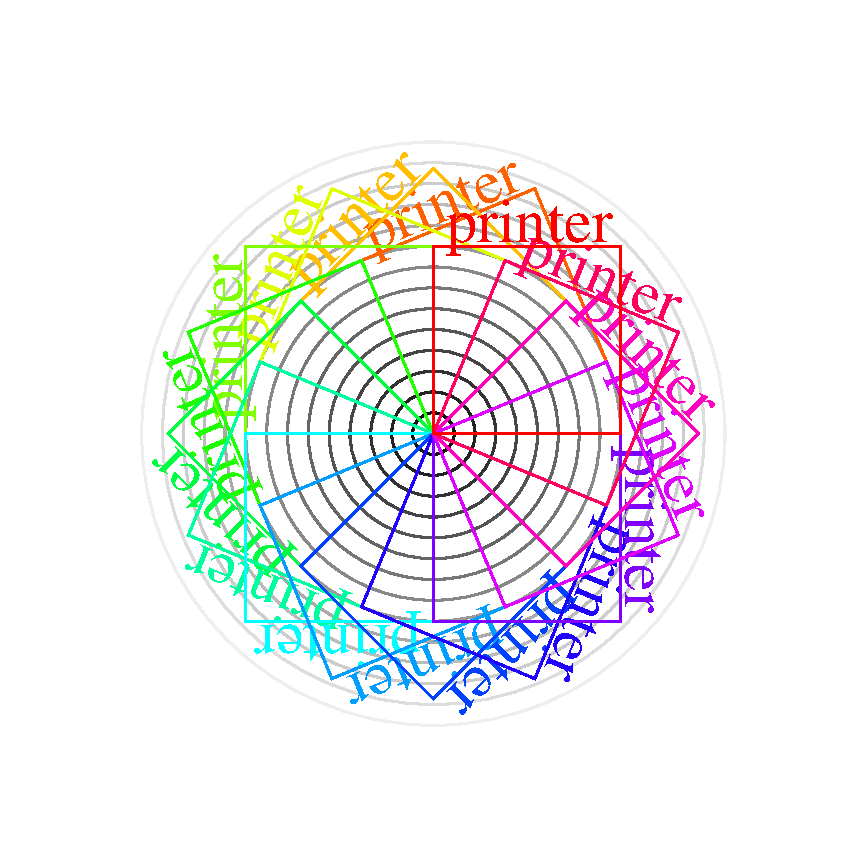
\includegraphics{figtestc.ps}
\label{figure4}
\end{figure}

Figure  \ref{figure4} tests \verb#\includegraphic{figtestc.ps}#.  

\end{document}
